\chapter{記分板}
\section{繪圖}
{
\begin{figure}[hbt!]
  \centering
  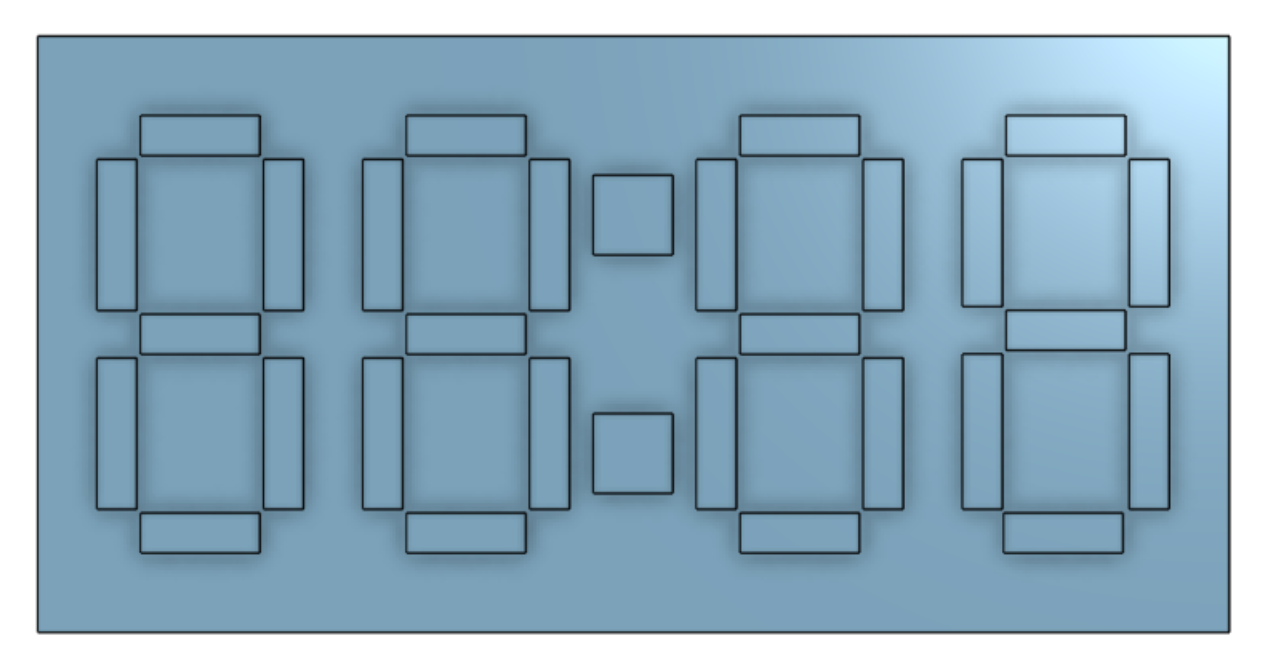
\includegraphics[width=0.5\textwidth]{計分板繪圖_17.png}
  \centering
  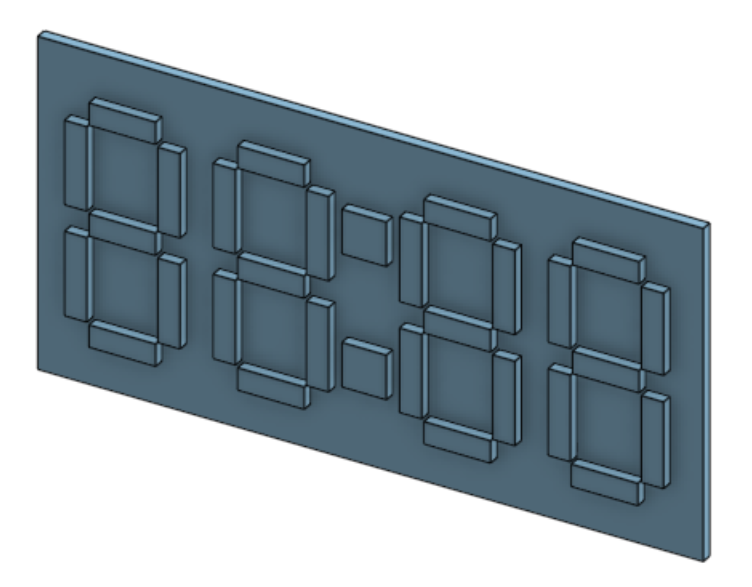
\includegraphics[width=0.5\textwidth]{計分板繪圖_18.png}
  \caption{LED記分板1}
  \label{fig:photo1}
\end{figure}

\begin{figure}[hbt!]
  \centering
  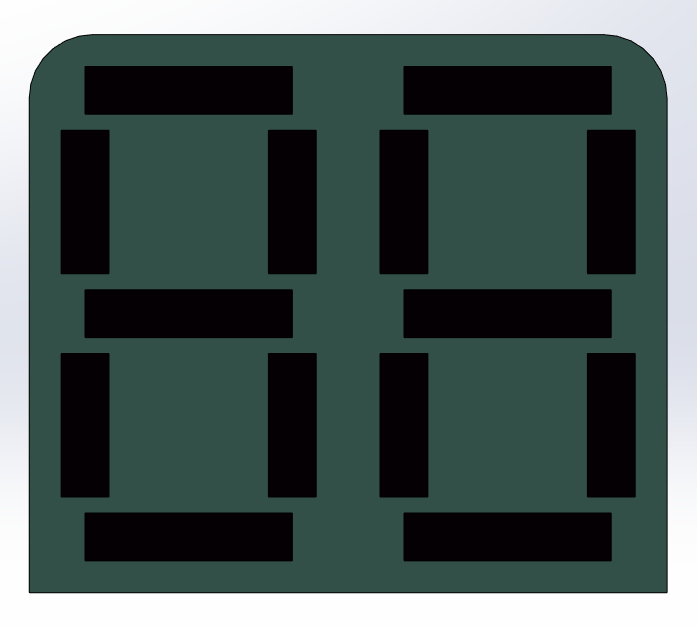
\includegraphics[width=0.5\textwidth]{計分板繪圖_15.png}
\end{figure}
\begin{figure}[hbt!]
  \centering
  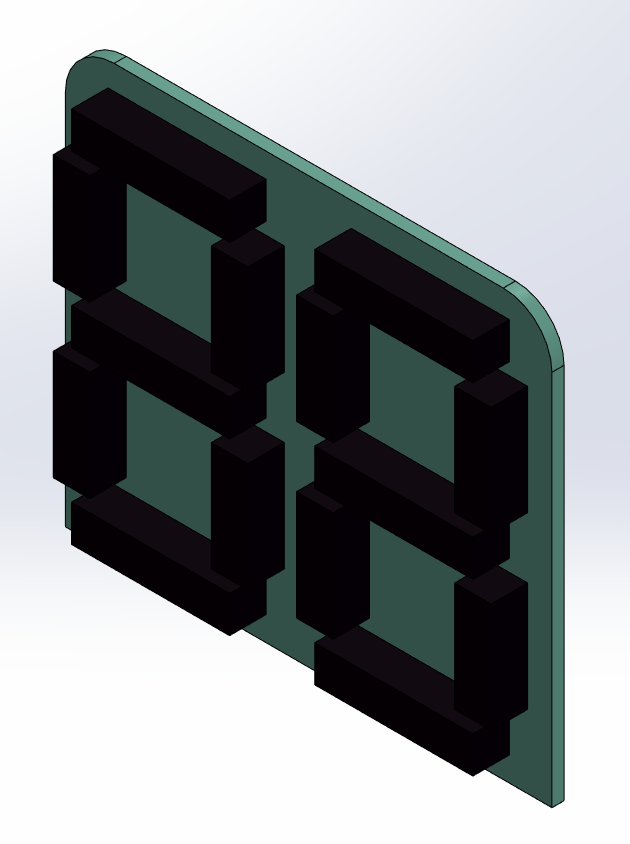
\includegraphics[width=0.5\textwidth]{計分板繪圖_16.png}
  \caption{LED記分板2}
  \label{fig:photo2}
\end{figure}

\begin{figure}[hbt!]
  \centering
  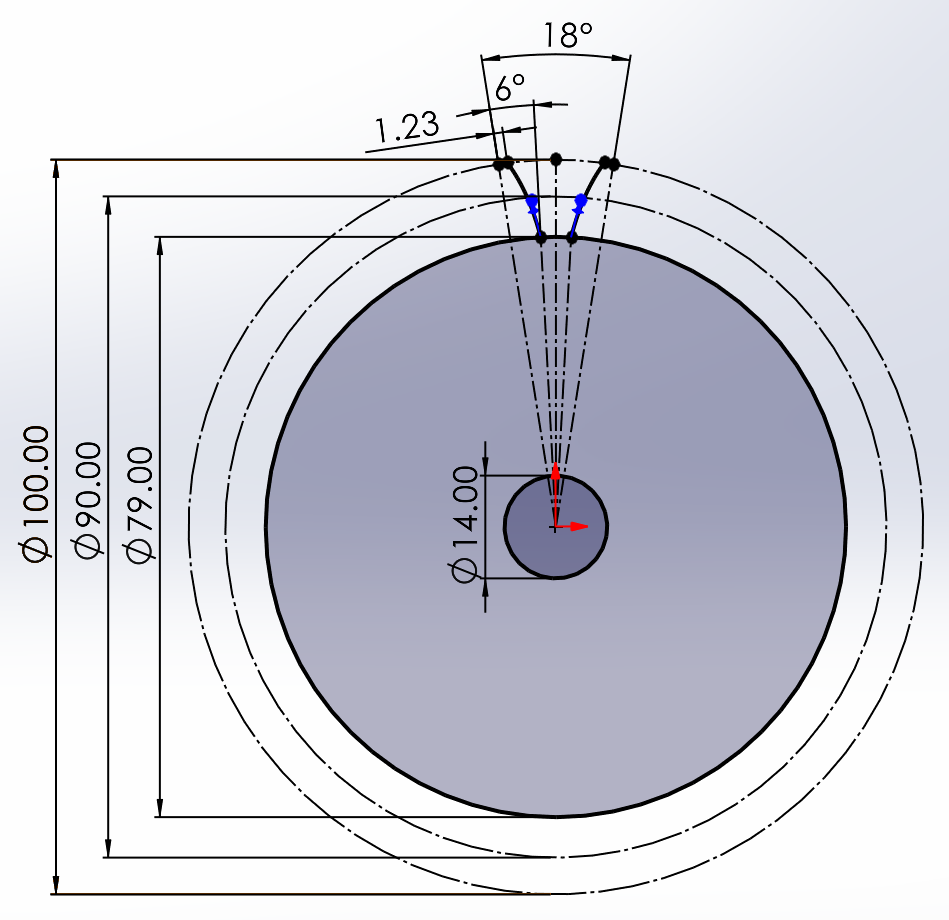
\includegraphics[width=0.5\textwidth]{計分板繪圖_1.png}
\end{figure}
\begin{figure}[hbt!]
  \centering
  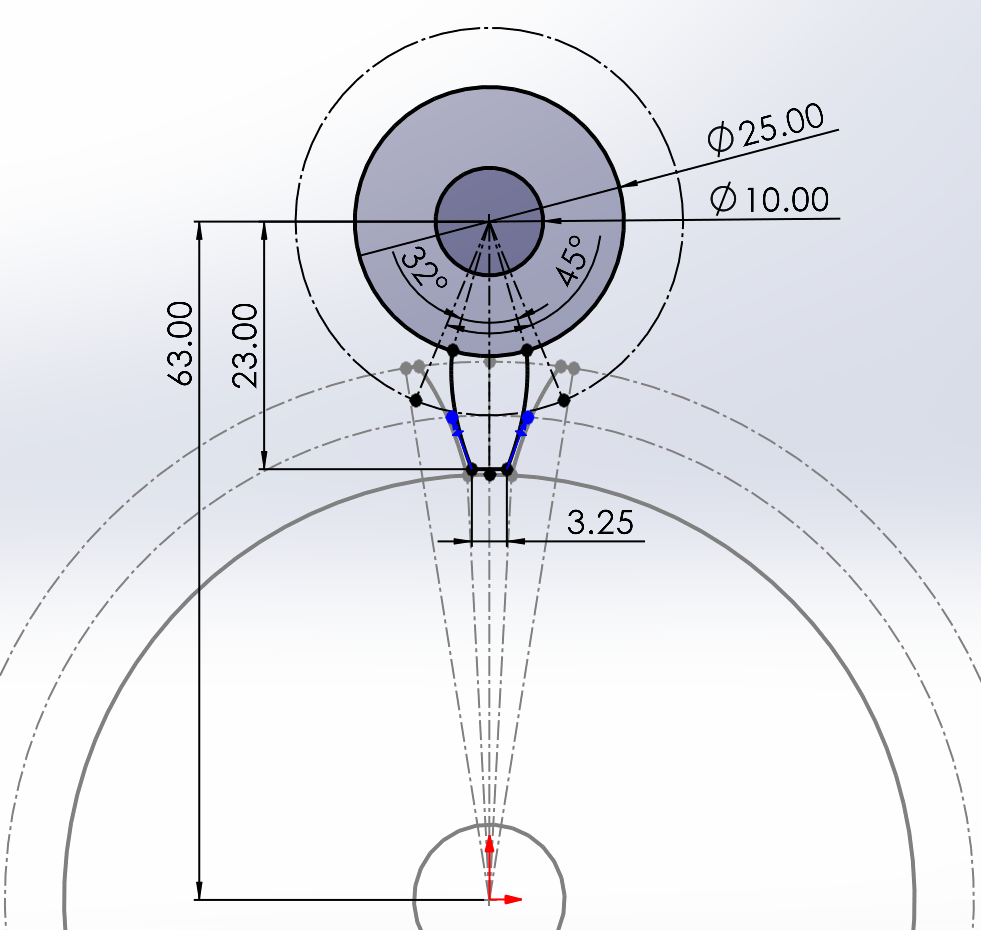
\includegraphics[width=0.5\textwidth]{計分板繪圖_2.png}
  \caption{sketch}
  \label{fig:photo3}
\end{figure}

\begin{figure}[hbt!]
  \centering
  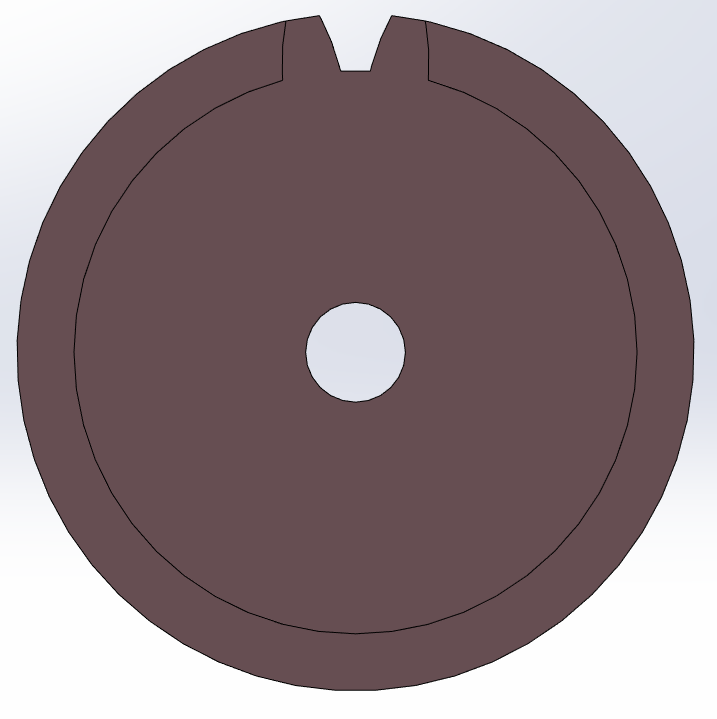
\includegraphics[width=0.5\textwidth]{計分板繪圖_3.png}
\end{figure}
\begin{figure}[hbt!]
  \centering
  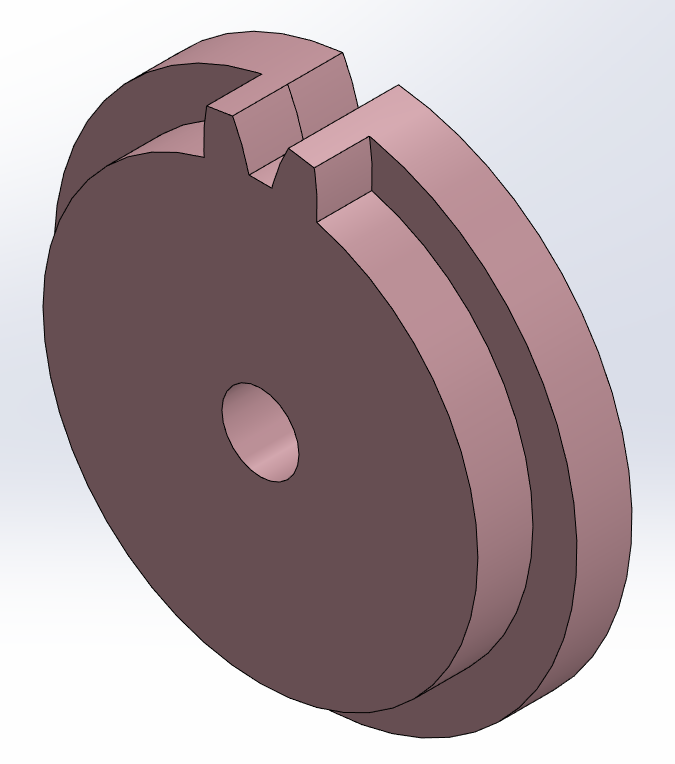
\includegraphics[width=0.5\textwidth]{計分板繪圖_4.png}
  \caption{Advancing Wheel gear}
  \label{fig:photo4}
\end{figure}

\begin{figure}[hbt!]
  \centering
  
\includegraphics[width=0.5\textwidth]{計分板繪圖_5.png}
\end{figure}
\begin{figure}[hbt!]
  \centering
  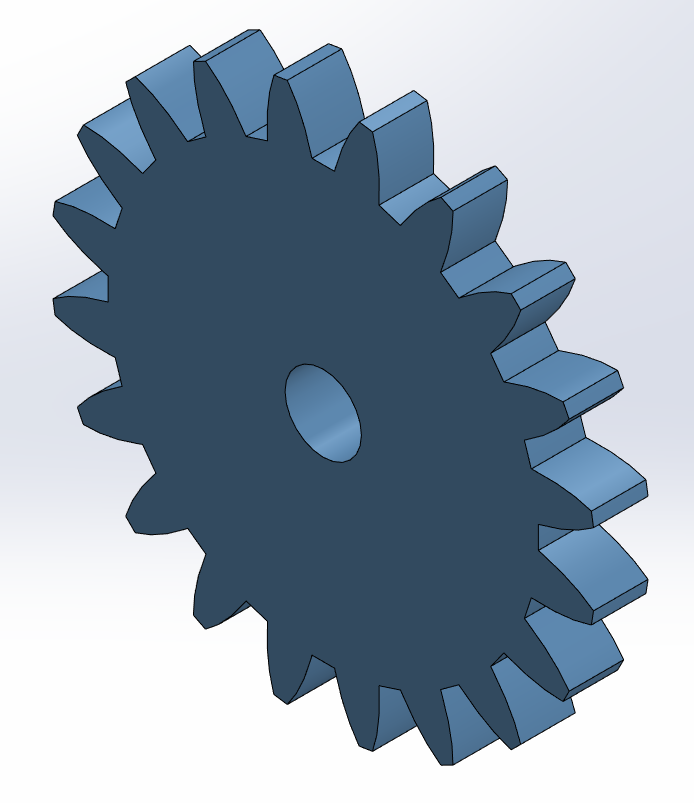
\includegraphics[width=0.5\textwidth]{計分板繪圖_6.png}
  \caption{M4.5 Teeth20 gear}
  \label{fig:photo5}
\end{figure}

\begin{figure}[hbt!]
  \centering
  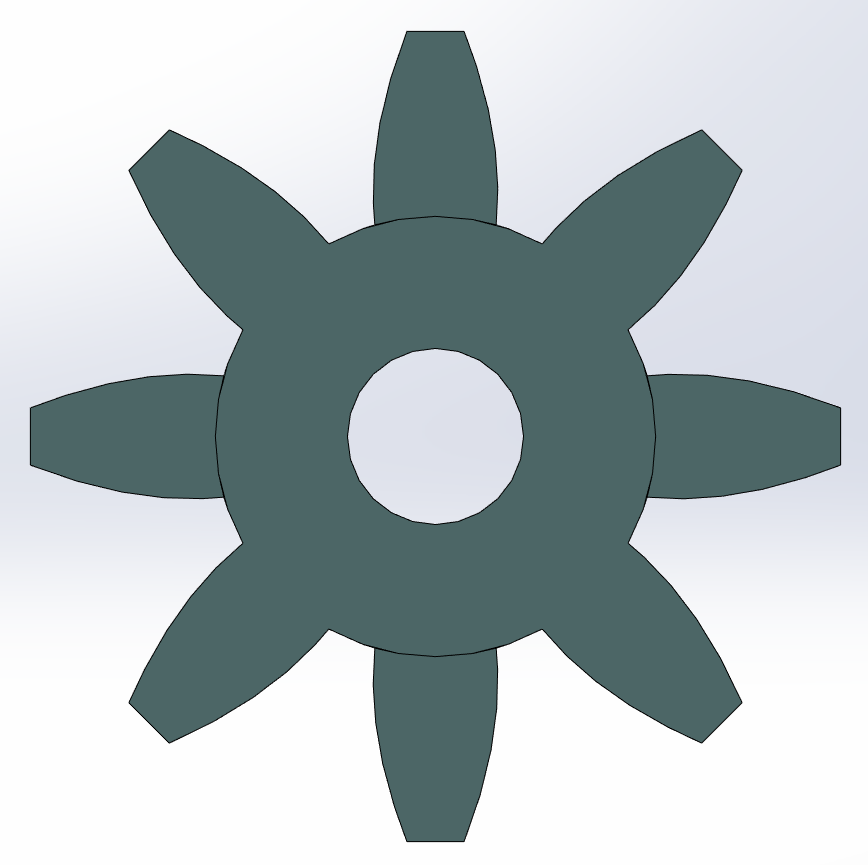
\includegraphics[width=0.5\textwidth]{計分板繪圖_7.png}
\end{figure}
\begin{figure}[hbt!]
  \centering
  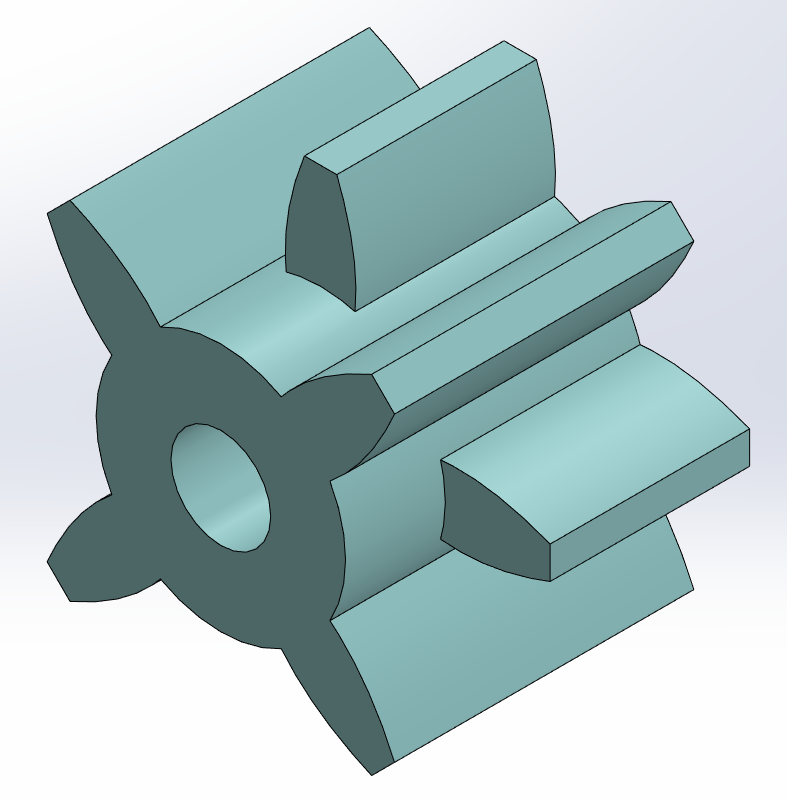
\includegraphics[width=0.5\textwidth]{計分板繪圖_8.png}
  \caption{M4.5 Teeth8 gear}
  \label{fig:photo6}
\end{figure}

\begin{figure}[hbt!]
  \centering
  
\includegraphics[width=0.5\textwidth]{計分板繪圖_11.png}
\end{figure}
\begin{figure}[hbt!]
  \centering
  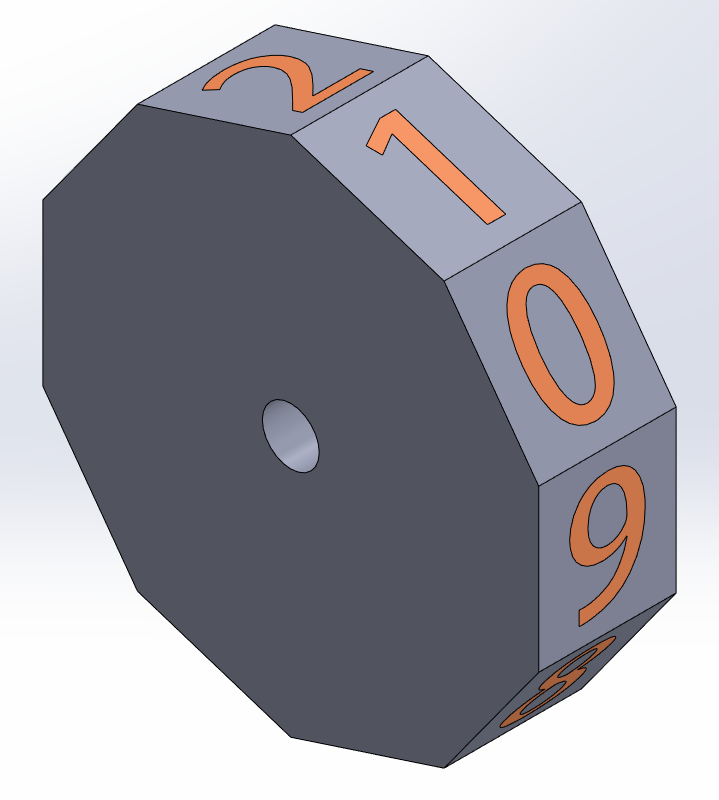
\includegraphics[width=0.5\textwidth]{計分板繪圖_12.png}
  \caption{Number Wheel}
  \label{fig:photo7}
\end{figure}

\begin{figure}[hbt!]
  \centering
  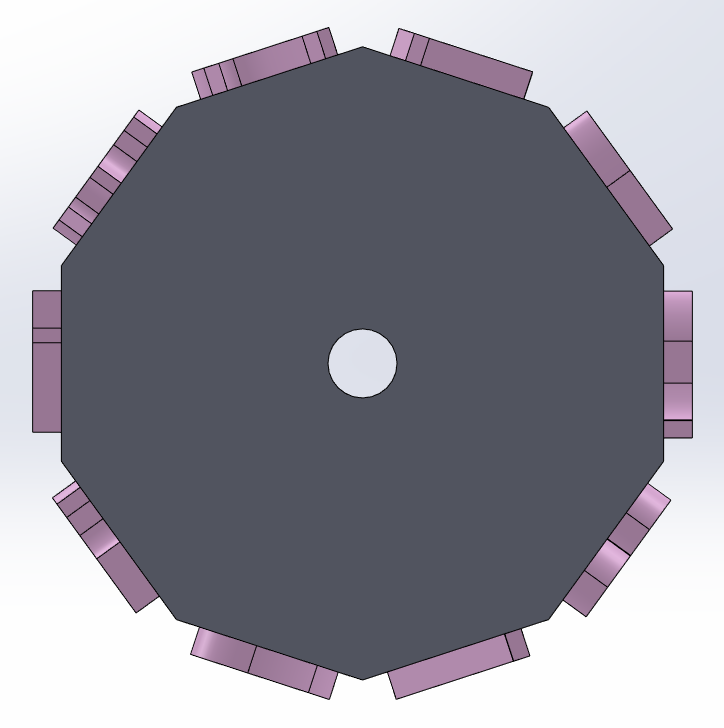
\includegraphics[width=0.5\textwidth]{計分板繪圖_9.png}
\end{figure}
\begin{figure}[hbt!]
  \centering
  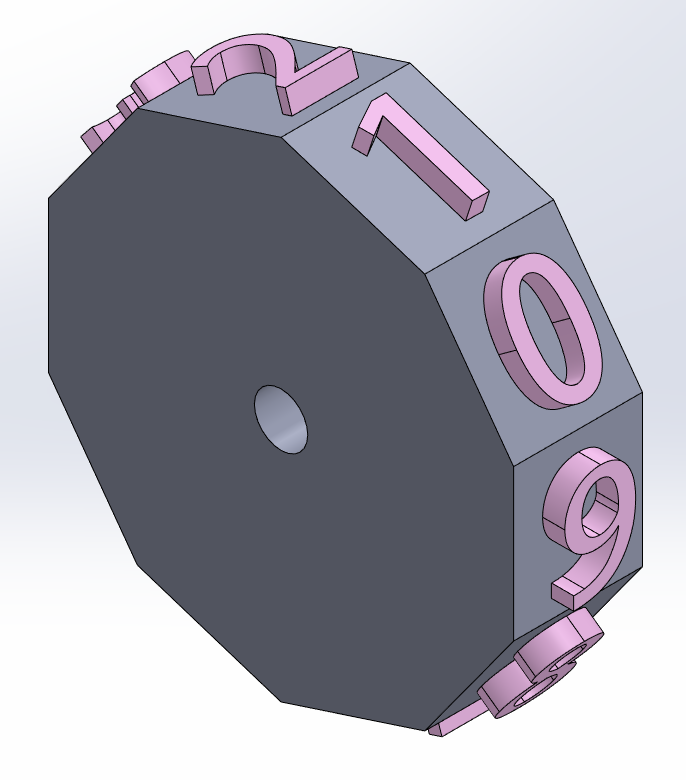
\includegraphics[width=0.5\textwidth]{計分板繪圖_10.png}
  \caption{Number Wheel1}
  \label{fig:photo8}
\end{figure}

\begin{figure}[hbt!]
  \centering
  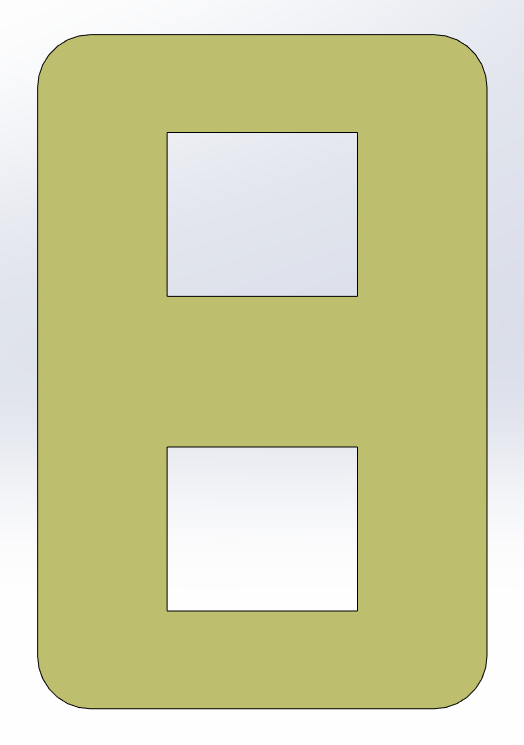
\includegraphics[width=0.5\textwidth]{計分板繪圖_13.png}
\end{figure}
\begin{figure}[hbt!]
  \centering
  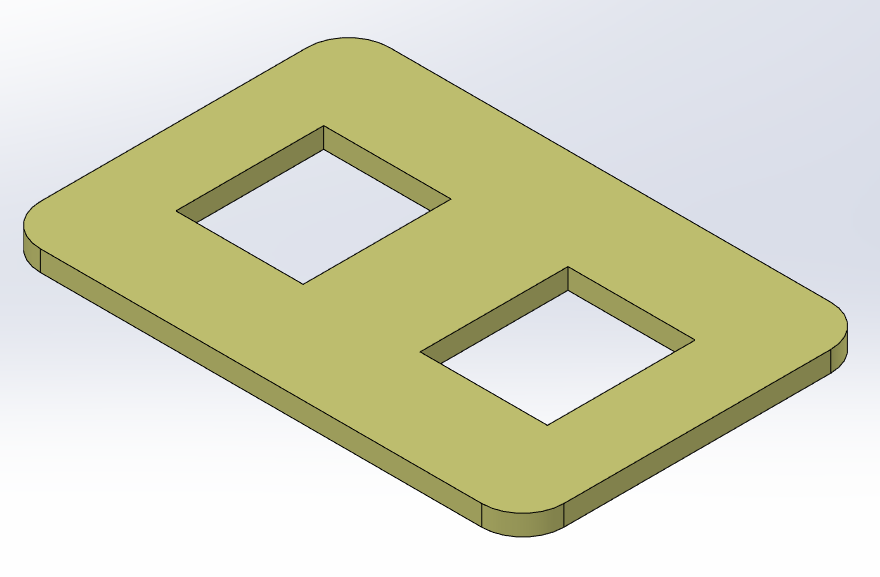
\includegraphics[width=0.5\textwidth]{計分板繪圖_14.png}
  \caption{board}
  \label{fig:photo9}
\end{figure}
}

\section{組合}
{
\begin{figure}[hbt!]
  \centering
  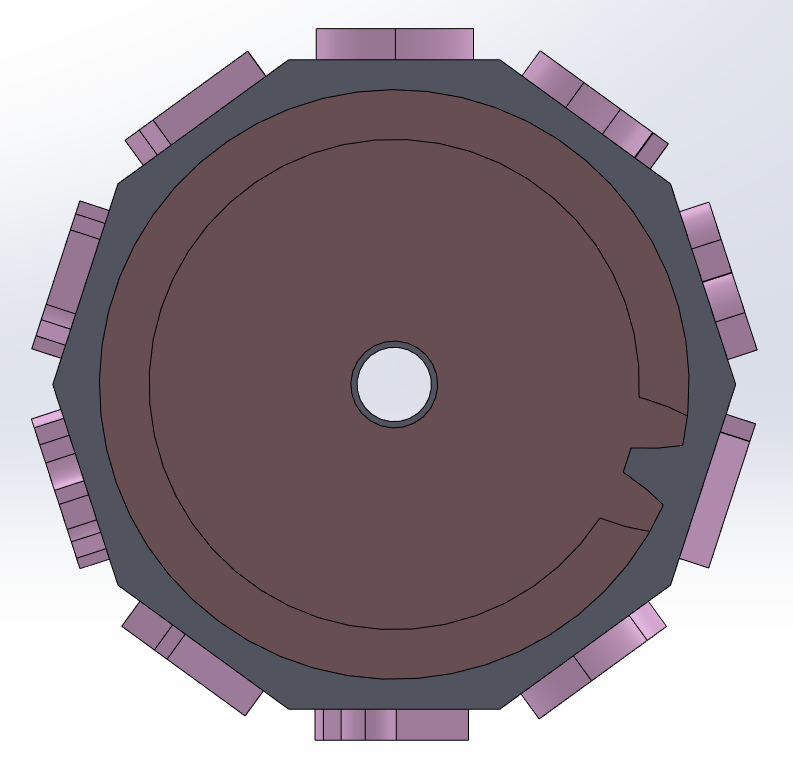
\includegraphics[width=0.5\textwidth]{計分板組合_1.png}
\end{figure}
\begin{figure}[hbt!]
  \centering
  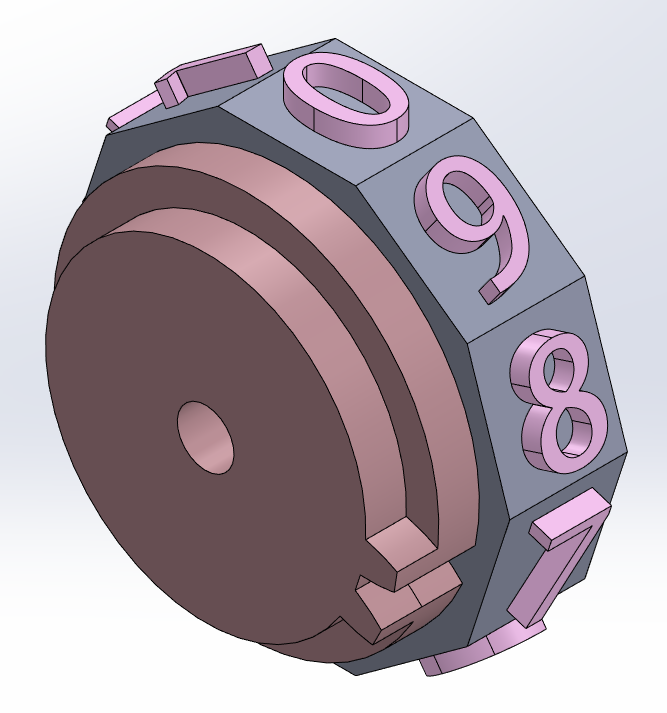
\includegraphics[width=0.5\textwidth]{計分板組合_2.png}
  \caption{Unit Digit Wheel}
  \label{fig:photo10}
\end{figure}

\begin{figure}[hbt!]
  \centering
  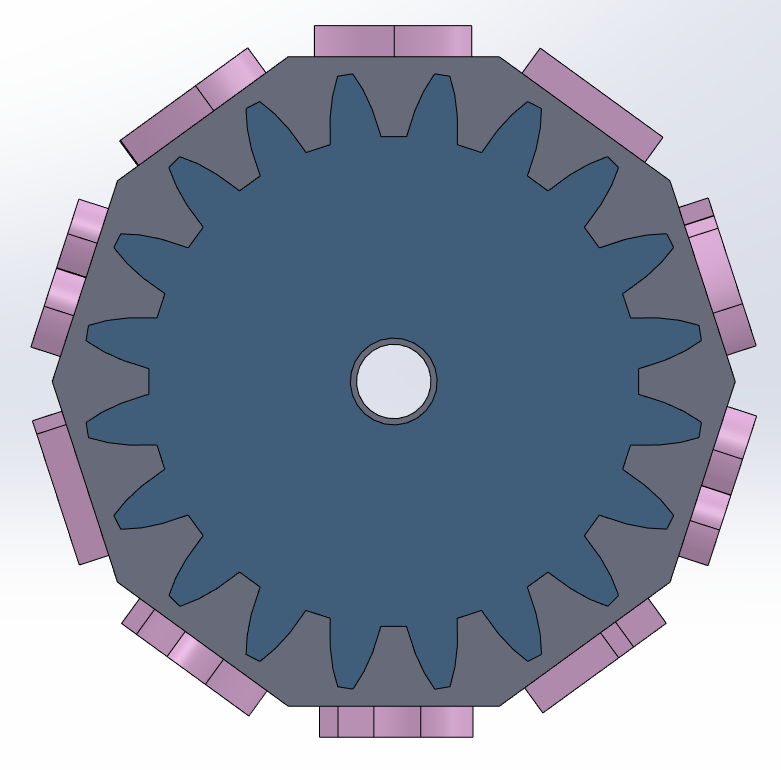
\includegraphics[width=0.5\textwidth]{計分板組合_3.png}
\end{figure}
\begin{figure}[hbt!]
  \centering
  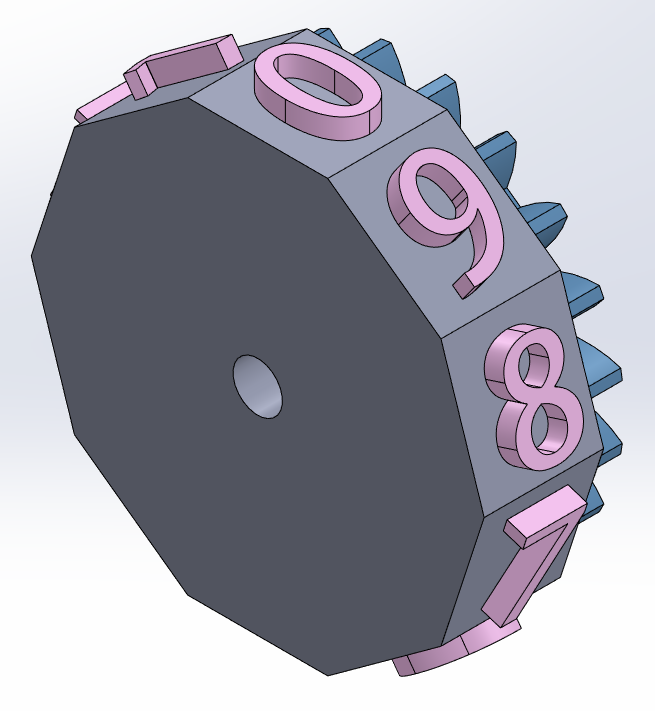
\includegraphics[width=0.5\textwidth]{計分板組合_4.png}
  \caption{Ten's Digit Wheel}
  \label{fig:photo11}
\end{figure}

\begin{figure}[hbt!]
  \centering
  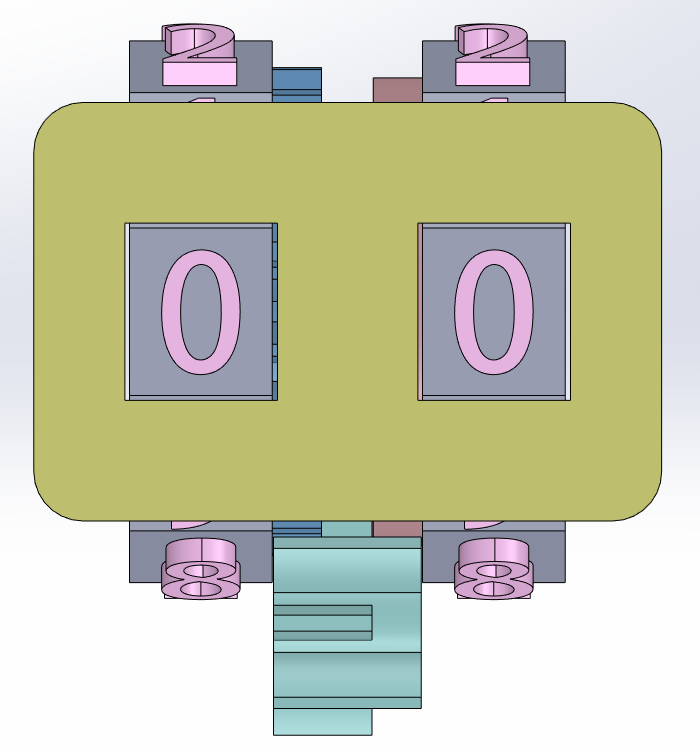
\includegraphics[width=0.5\textwidth]{計分板組合_5.png}
\end{figure}
\begin{figure}[hbt!]
  \centering
  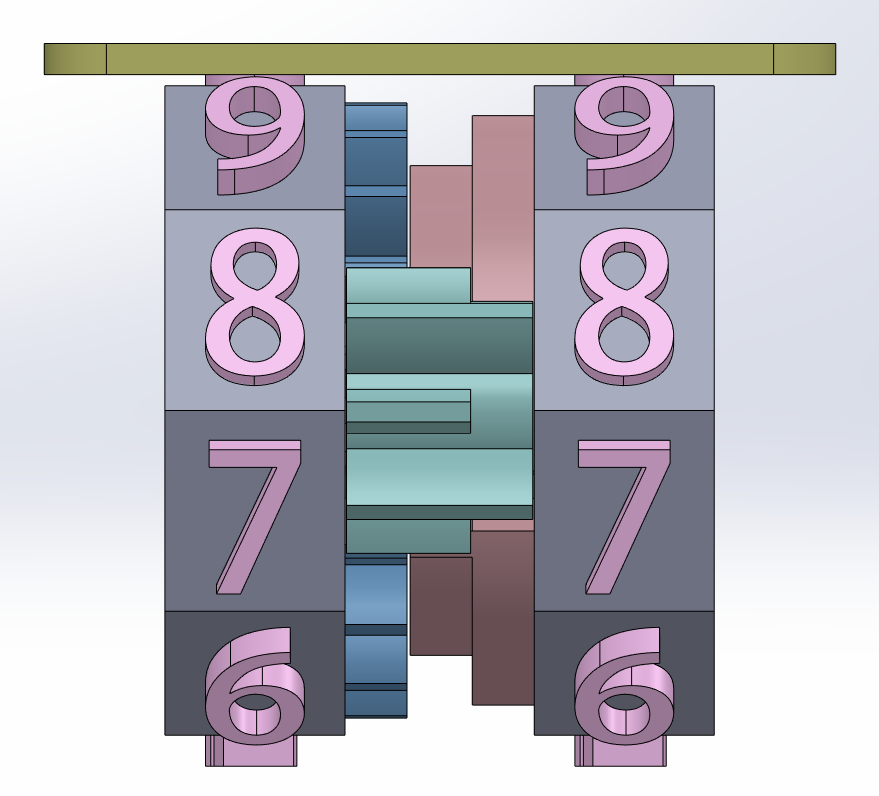
\includegraphics[width=0.5\textwidth]{計分板組合_6.png}
\end{figure}
\begin{figure}[hbt!]
  \centering
  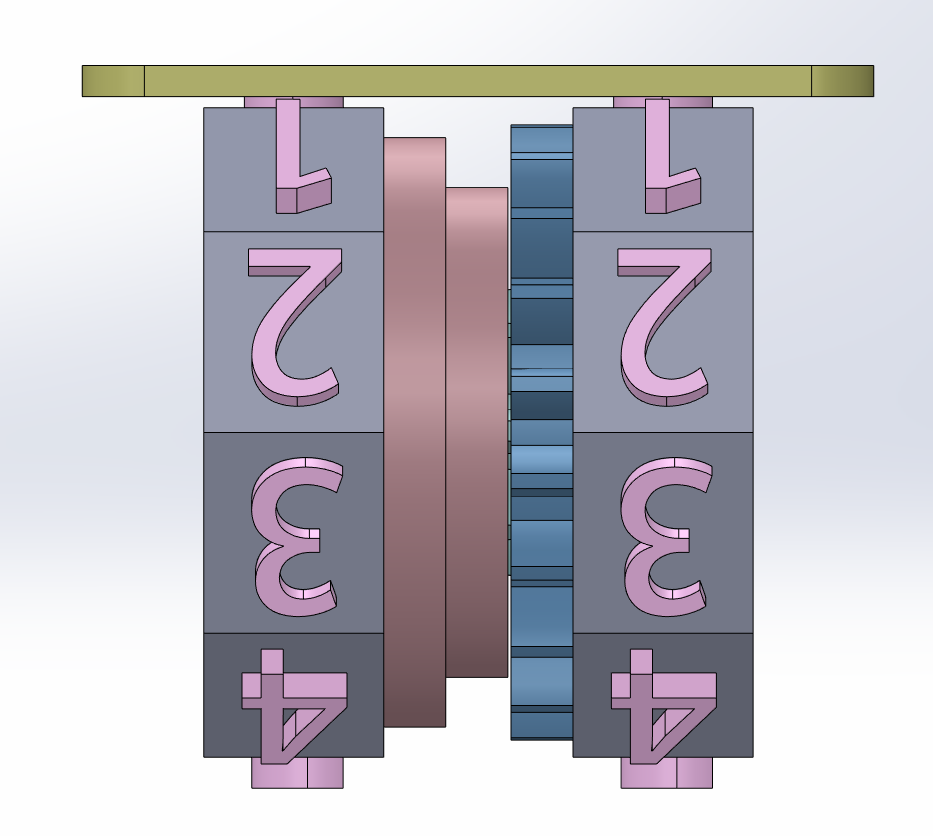
\includegraphics[width=0.5\textwidth]{計分板組合_7.png}
\end{figure}
\begin{figure}[hbt!]
  \centering
  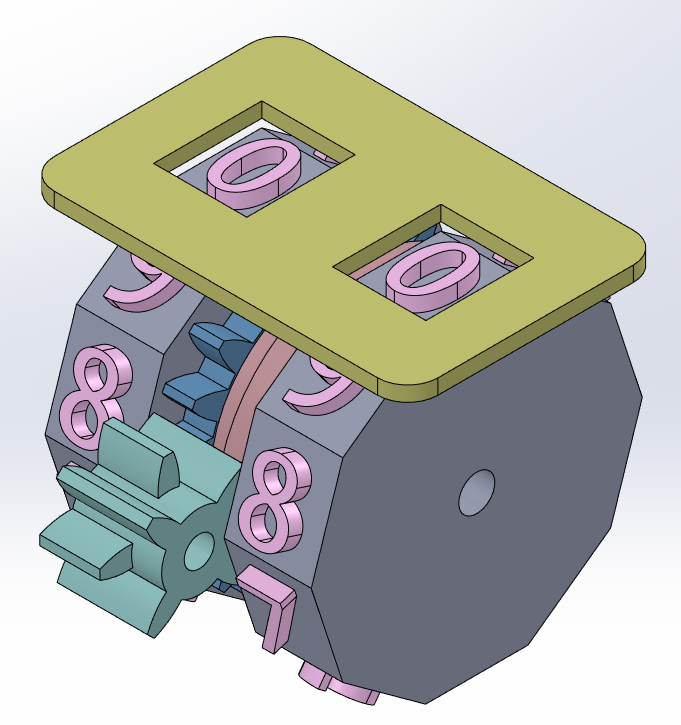
\includegraphics[width=0.5\textwidth]{計分板組合_8.png}
  \caption{Mechanical Counter}
  \label{fig:photo12}
\end{figure}
}

\section{組裝}
{
\begin{figure}[hbt!]
  \centering
  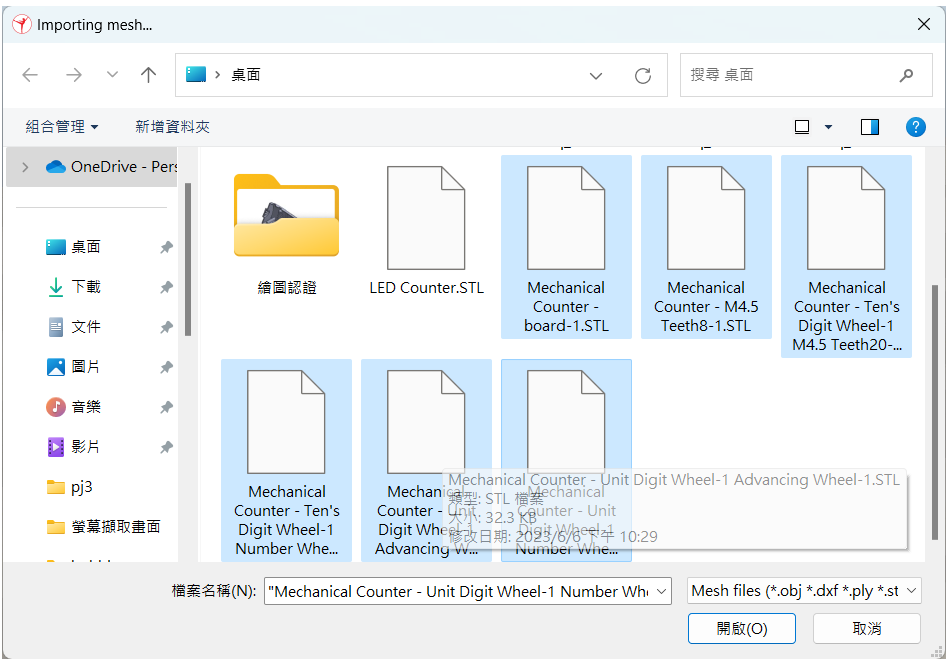
\includegraphics[width=0.5\textwidth]{記分板組裝_1.png}
\end{figure}
\begin{figure}[hbt!]
  \centering
  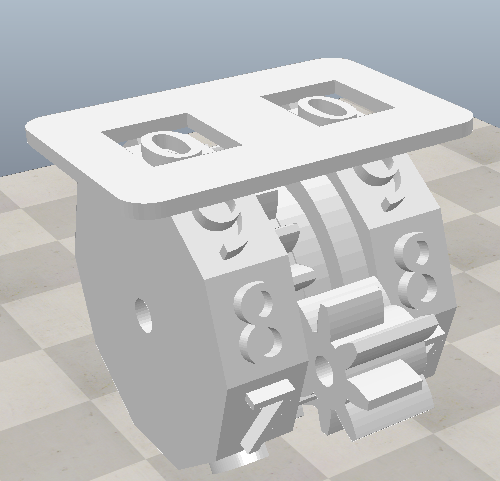
\includegraphics[width=0.5\textwidth]{記分板組裝_2.png}
  \caption{一次選取所有STL檔導入}
  \label{fig:photo13}
\end{figure}

\begin{figure}[hbt!]
  \begin{center}
    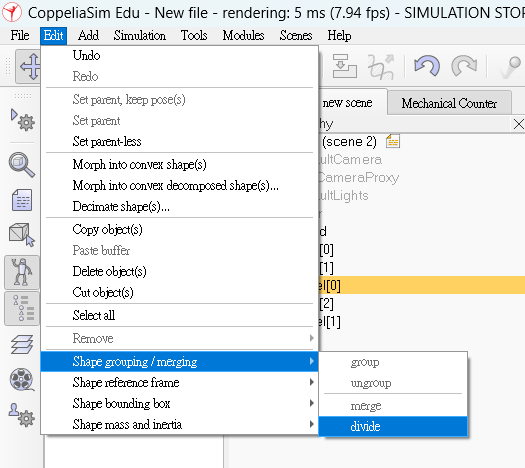
\includegraphics[width=0.5\textwidth]{記分板組裝_3.png}
  \end{center}
  \caption{將wheel物件爆炸分解}
  \label{fig:photo}
\end{figure}

\begin{figure}[hbt!]
  \begin{center}
    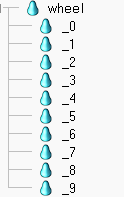
\includegraphics[width=0.5\textwidth]{記分板組裝_4.png}
  \end{center}
  \caption{更改數字名稱}
  \label{fig:photo}
\end{figure}

\begin{figure}[hbt!]
  \begin{center}
    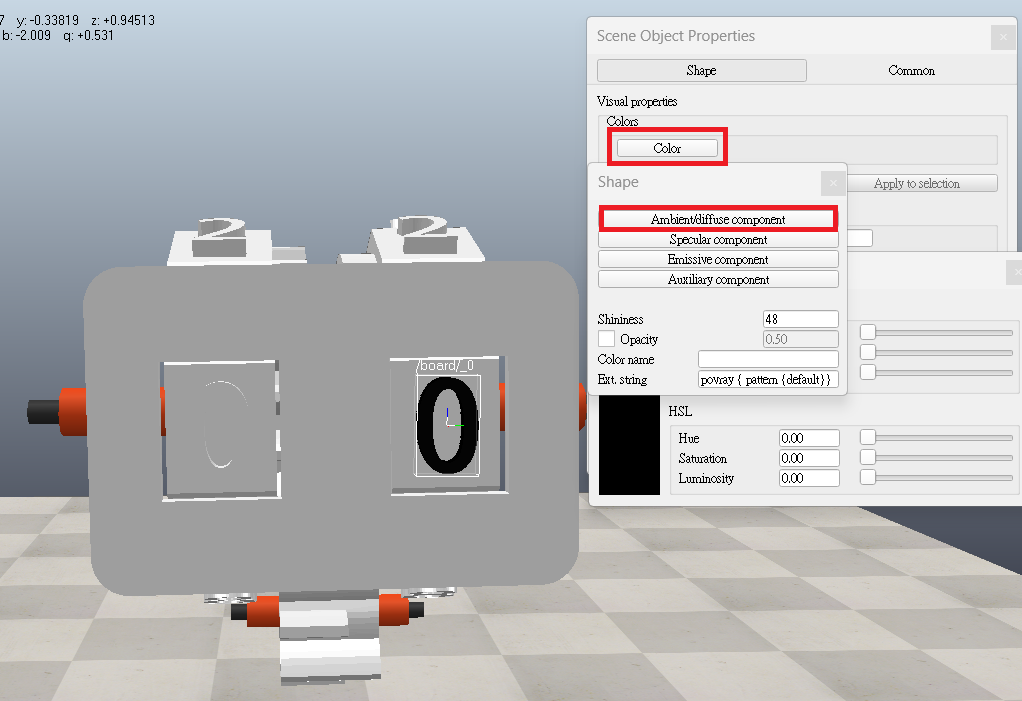
\includegraphics[width=0.5\textwidth]{記分板組裝_5.png}
  \end{center}
  \caption{更改數字顏色}
  \label{fig:photo}
\end{figure}

\begin{figure}[hbt!]
  \begin{center}
    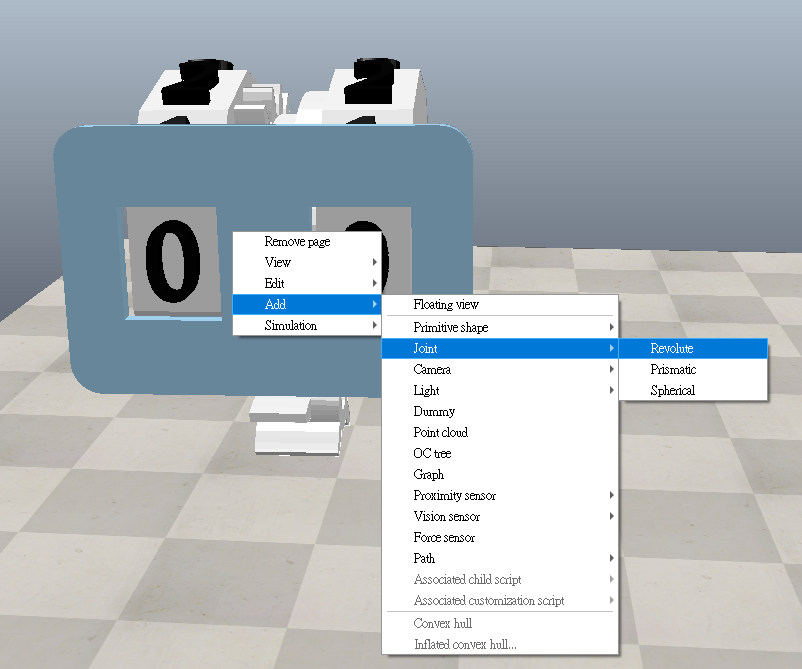
\includegraphics[width=0.5\textwidth]{記分板組裝_8.png}
  \end{center}
  \caption{新增Joint}
  \label{fig:photo}
\end{figure}

\begin{figure}[hbt!]
  \begin{center}
    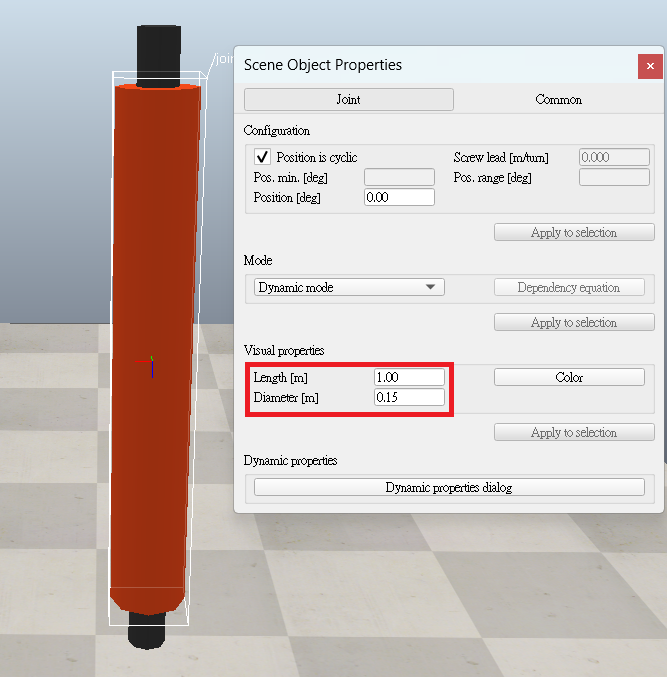
\includegraphics[width=0.5\textwidth]{記分板組裝_9.png}
  \end{center}
  \caption{調整Joint方向及大小}
  \label{fig:photo}
\end{figure}

\begin{figure}[hbt!]
  \begin{center}
    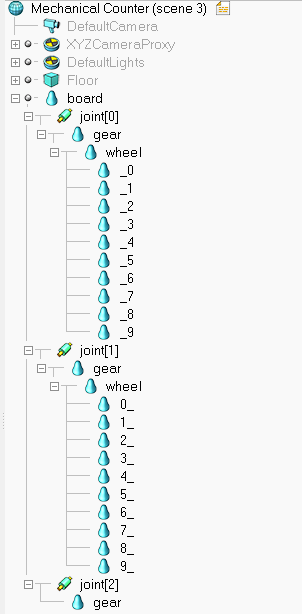
\includegraphics[width=0.5\textwidth]{記分板組裝_7.png}
  \end{center}
  \caption{物件相互依附}
  \label{fig:photo}
\end{figure}

\begin{figure}[hbt!]
  \begin{center}
    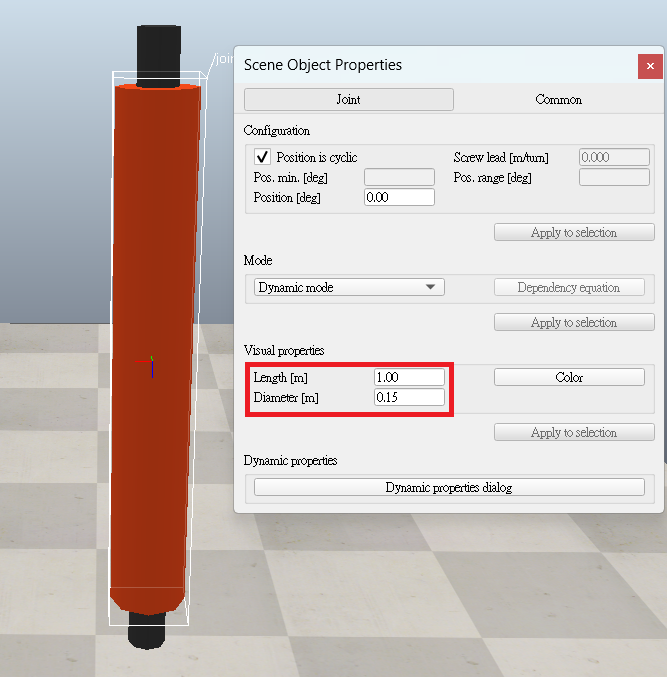
\includegraphics[width=0.5\textwidth]{記分板組裝_9.png}
  \end{center}
  \caption{調整Joint方向及大小}
  \label{fig:photo}
\end{figure}

\begin{figure}[hbt!]
  \begin{center}
    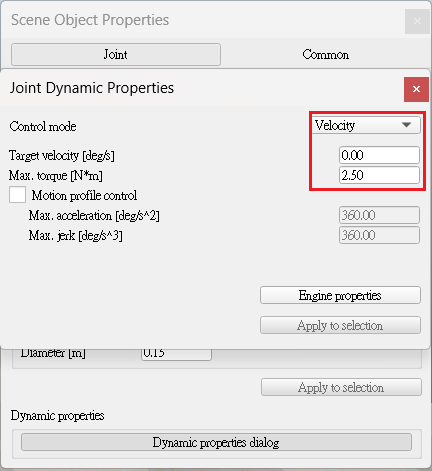
\includegraphics[width=0.5\textwidth]{記分板組裝_10.png}
  \end{center}
  \caption{調整物件傳動參數}
  \label{fig:photo}
\end{figure}

\begin{figure}[hbt!]
  \begin{center}
    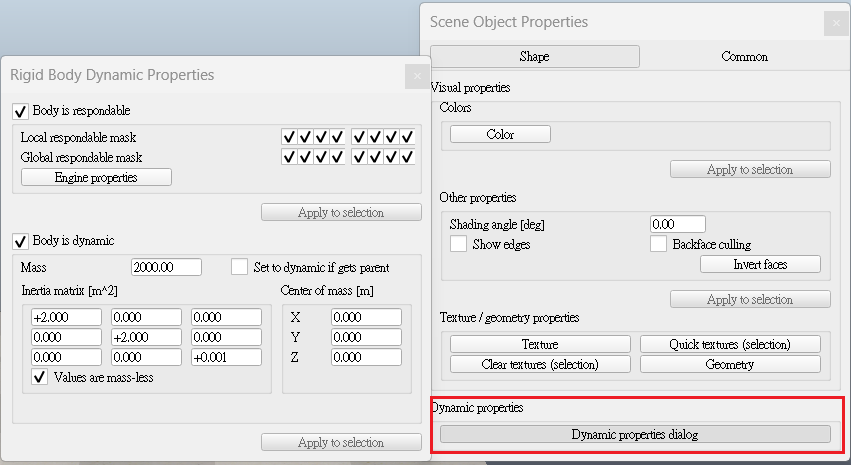
\includegraphics[width=0.5\textwidth]{記分板組裝_11.png}
  \end{center}
  \caption{調整物件質量參數}
  \label{fig:photo}
\end{figure}

\begin{figure}[hbt!]
  \begin{center}
    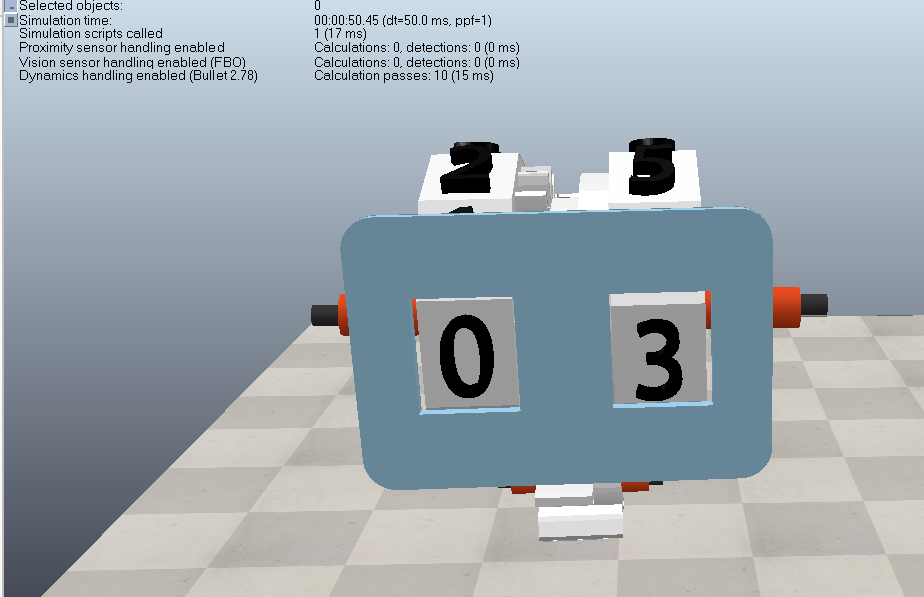
\includegraphics[width=0.5\textwidth]{記分板組裝_12.png}
  \end{center}
  \caption{完成記分板}
  \label{fig:photo}
\end{figure}
}
